\documentclass[tikz,border=8pt]{standalone}
% Shared look for every TikZ diagram. Load with \input{../../tools/tikz-style.tex}
\usepackage[T1]{fontenc}
\usepackage{lmodern}
\renewcommand{\sfdefault}{lmr}  % diagrams use the same serif as the text
\usetikzlibrary{arrows.meta, positioning, shapes.geometric, calc, fit, backgrounds}
\definecolor{cblue}{HTML}{4C78A8}
\definecolor{corange}{HTML}{F58518}
\definecolor{cgreen}{HTML}{54A24B}
\definecolor{cred}{HTML}{E45756}
\definecolor{cpurple}{HTML}{B279A2}
\definecolor{cgrey}{HTML}{6B6B6B}
\tikzset{
  every picture/.style={font=\sffamily, line width=1.2pt},
  box/.style={draw=#1, fill=#1!12, rounded corners=4pt, align=center, inner sep=7pt, minimum height=1.1cm},
  box/.default=cgrey,
  arrow/.style={-{Stealth[length=3mm]}, draw=cgrey, line width=1.4pt},
  title/.style={font=\sffamily\bfseries\Large},
  note/.style={font=\sffamily\small, text=cgrey, align=center},
}
\AtBeginDocument{\hyphenpenalty=10000 \exhyphenpenalty=10000}

% Resampling the five particles of the worked example. Their normalised weights 0.0031, 0.3313, 0.3313, 0.0031,
% 0.3313 split the line from 0 to 1 into five stretches. Top: the low-variance sampler, one random start r = 0.12,
% then pointers every 1/5 = 0.2: copies 0, 2, 1, 0, 2. Bottom: five independent random numbers
% (0.33, 0.99, 0.32, 0.79, 0.87): copies 0, 2, 0, 0, 3, so particle 3 is lost.
\begin{document}
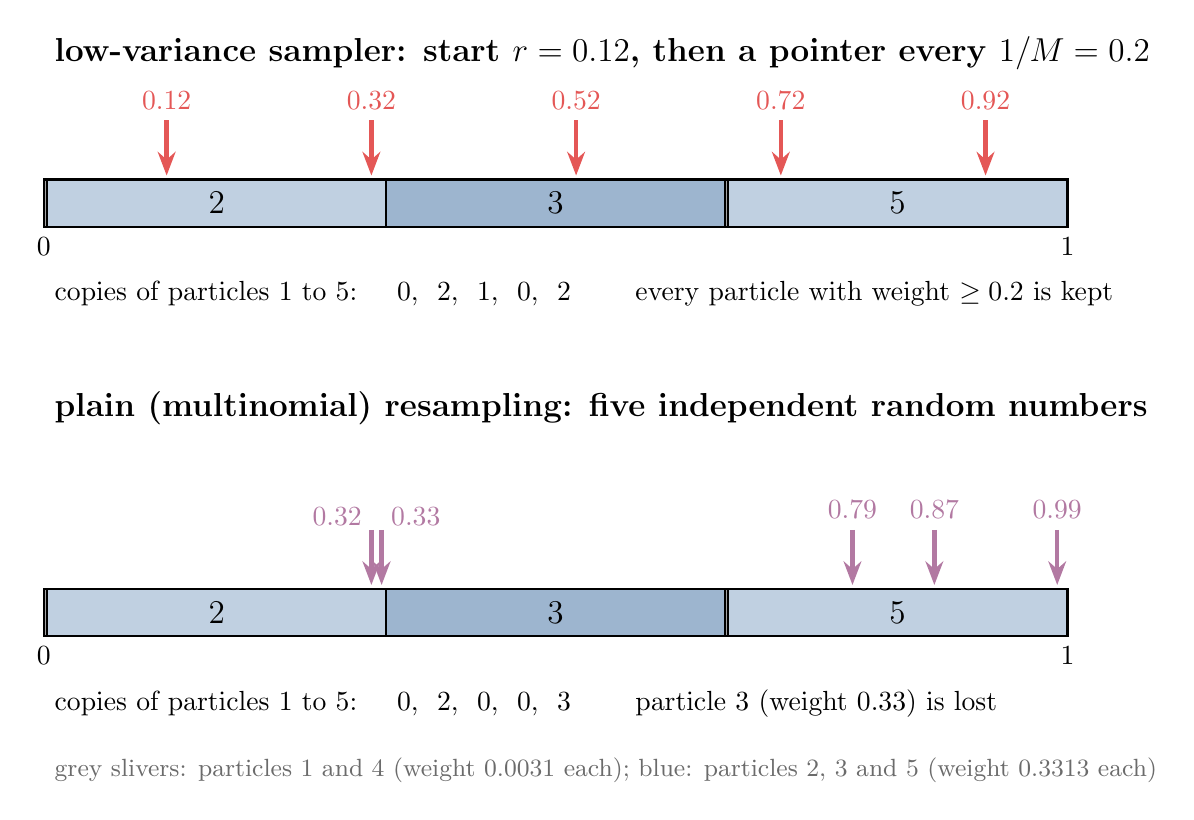
\begin{tikzpicture}[x=13cm, y=1cm, every node/.append style={font=\large}]
  \newcommand{\weightbar}{%
    \fill[cgrey!60] (0,0) rectangle (0.0031,0.6);
    \fill[cblue!35] (0.0031,0) rectangle (0.3344,0.6);
    \fill[cblue!55] (0.3344,0) rectangle (0.6656,0.6);
    \fill[cgrey!60] (0.6656,0) rectangle (0.6687,0.6);
    \fill[cblue!35] (0.6687,0) rectangle (1,0.6);
    \draw[black, line width=0.8pt] (0,0) rectangle (1,0.6);
    \foreach \t in {0.0031,0.3344,0.6656,0.6687} \draw[black, line width=0.8pt] (\t,0) -- (\t,0.6);
    \node at (0.169,0.3) {2};
    \node at (0.500,0.3) {3};
    \node at (0.834,0.3) {5};
    \node[below, font=\normalsize] at (0,0) {0};
    \node[below, font=\normalsize] at (1,0) {1};
  }
  % ---- low-variance sampler
  \node[anchor=west, font=\large\bfseries] at (0,2.2) {low-variance sampler: start $r = 0.12$, then a pointer every $1/M = 0.2$};
  \begin{scope}[shift={(0,0)}]
    \weightbar
    \foreach \p in {0.12,0.32,0.52,0.72,0.92} {
      \draw[-{Stealth[length=3mm]}, cred, line width=1.6pt] (\p,1.35) -- (\p,0.65);
      \node[cred, above, font=\normalsize] at (\p,1.35) {\p};
    }
    \node[anchor=west, font=\normalsize] at (0,-0.85) {copies of particles 1 to 5: \quad 0, \ 2, \ 1, \ 0, \ 2 \qquad every particle with weight $\geq 0.2$ is kept};
  \end{scope}
  % ---- multinomial
  \node[anchor=west, font=\large\bfseries] at (0,-2.3) {plain (multinomial) resampling: five independent random numbers};
  \begin{scope}[shift={(0,-5.2)}]
    \weightbar
    \foreach \p in {0.33,0.32,0.79,0.87,0.99} \draw[-{Stealth[length=3mm]}, cpurple, line width=1.6pt] (\p,1.35) -- (\p,0.65);
    \node[cpurple, above right, font=\normalsize, inner sep=1pt] at (0.335,1.35) {0.33};
    \node[cpurple, above left, font=\normalsize, inner sep=1pt] at (0.315,1.35) {0.32};
    \foreach \p in {0.79,0.87,0.99} \node[cpurple, above, font=\normalsize] at (\p,1.35) {\p};
    \node[anchor=west, font=\normalsize] at (0,-0.85) {copies of particles 1 to 5: \quad 0, \ 2, \ 0, \ 0, \ 3 \qquad particle 3 (weight 0.33) is lost};
  \end{scope}
  \node[note, anchor=west] at (0,-6.9) {grey slivers: particles 1 and 4 (weight 0.0031 each); blue: particles 2, 3 and 5 (weight 0.3313 each)};
\end{tikzpicture}
\end{document}
